\documentclass[11pt,a4paper]{article}
\usepackage[margin=2.2cm]{geometry}
\usepackage{amsmath,amssymb,bm}
\usepackage{graphicx,float,booktabs,caption,subcaption}
\usepackage{xcolor}
\usepackage{listings}
\usepackage{tikz}
\usetikzlibrary{shapes.geometric,arrows.meta,positioning,calc}
\usepackage[colorlinks=true,linkcolor=blue!50!black,urlcolor=blue!50!black,citecolor=blue!50!black]{hyperref}
\usepackage{fancyhdr}
\pagestyle{fancy}\fancyhf{}\lhead{\small Karthick J (OE23S018), IIT Madras}\rhead{\small\leftmark}\cfoot{\thepage}
\definecolor{codebg}{rgb}{0.97,0.97,0.97}
\lstset{basicstyle=\ttfamily\scriptsize,backgroundcolor=\color{codebg},frame=single,breaklines=true,
 keywordstyle=\color{blue!60!black}\bfseries,commentstyle=\color{green!40!black},stringstyle=\color{red!50!black},
 numbers=left,numberstyle=\tiny\color{gray},showstringspaces=false,tabsize=4,columns=fullflexible,
 literate={²}{{$^2$}}1 {³}{{$^3$}}1 {°}{{$^\circ$}}1 {Δ}{{$\Delta$}}1 {ρ}{{$\rho$}}1 {μ}{{$\mu$}}1 {ω}{{$\omega$}}1 {ψ}{{$\psi$}}1 {α}{{$\alpha$}}1 {ν}{{$\nu$}}1 {τ}{{$\tau$}}1 {–}{{-}}1 {—}{{-}}1 {’}{{'}}1 {“}{{"}}1 {”}{{"}}1 {→}{{$\to$}}1 {≤}{{$\le$}}1 {≥}{{$\ge$}}1 {×}{{$\times$}}1 {±}{{$\pm$}}1 {·}{{$\cdot$}}1 {∂}{{$\partial$}}1 {∇}{{$\nabla$}}1 {γ}{{$\gamma$}}1 {ε}{{$\varepsilon$}}1 {μ}{{$\mu$}}1 {├}{{+}}1 {─}{{-}}1 {│}{{|}}1 {▶}{{>}}1 {▼}{{v}}1 {┌}{{+}}1 {┐}{{+}}1 {└}{{+}}1 {┘}{{+}}1 {┬}{{+}}1 {┴}{{+}}1}
\tikzset{
 startstop/.style={rectangle,rounded corners=6pt,minimum width=3.2cm,minimum height=0.8cm,text centered,draw=black,fill=red!12,font=\small},
 process/.style={rectangle,minimum width=4.6cm,minimum height=0.8cm,text centered,text width=5.6cm,draw=black,fill=blue!8,font=\small},
 decision/.style={diamond,aspect=2.6,text centered,text width=3.2cm,draw=black,fill=green!12,font=\small,inner sep=1pt},
 io/.style={trapezium,trapezium left angle=72,trapezium right angle=108,minimum width=3.6cm,minimum height=0.8cm,text centered,text width=4.6cm,draw=black,fill=orange!15,font=\small},
 arrow/.style={thick,-{Stealth[length=2.5mm]}}}
\setlength{\parskip}{4pt}\setlength{\parindent}{0pt}

\title{\textbf{GPU-Parallel Lid-Driven Cavity Solver}\\[2pt]\large Vorticity--Stream Function Formulation of the 2-D Navier--Stokes Equations in CUDA C\\[2pt]\normalsize Course Project 2 -- OE5450 Numerical Techniques in Ocean Hydrodynamics (Tutorial 6, Jan--May 2025)}
\author{Karthick J (OE23S018)\\Department of Ocean Engineering, IIT Madras}
\date{Revised report, October 2026}
\begin{document}\maketitle
\begin{abstract}
The steady flow in a lid-driven square cavity at $\mathrm{Re}=100$ is computed with an explicit vorticity--stream function finite-difference method whose four stencil operations (Thom wall vorticity, vorticity transport, red--black Gauss--Seidel stream-function relaxation and velocity recovery) are CUDA kernels with one thread per grid node. The submitted code could not produce a result: its time step was 6.4 times above the explicit diffusion limit derived in the original handwritten notes ($\Delta t\le h^2\mathrm{Re}/4$), so the vorticity overflowed within a dozen steps; it also wrote one 11 MB file per time step, and the output and velocity routines indexed the arrays transposed. With these errors corrected (and the steady-state tolerance scaled with the time step), the unmodified kernels were verified on three grids ($129^2$, $257^2$, $401^2$) by running them serially on the CPU through a CUDA emulation layer. The primary vortex ($\psi_{min}=-0.10350$ at $(0.616,0.737)$) and the centreline velocities agree with Ghia et al.\ (1982) within the accuracy of that benchmark; a three-grid study gives an observed order of accuracy of $2.01$--$2.02$ for $\psi_{min}$, $u_{min}$, $v_{max}$ and $v_{min}$, Richardson-extrapolated values $\psi_{min}=-0.10352$, $u_{min}=-0.21405$, $v_{max}=0.17957$, $v_{min}=-0.25380$, and a grid convergence index below $0.05\%$ on the finest grid. \texttt{run.sh} repeats all runs on an NVIDIA GPU when one is present and records the GPU wall times next to the single-core baseline reported here.
\end{abstract}
\tableofcontents\newpage

\section{Problem definition}
A unit square cavity, $0\le x,y\le1$, is filled with an incompressible Newtonian fluid; the lid $y=1$ moves with $U=1$ and the other walls are at rest. In two dimensions the Navier--Stokes equations can be written for the vorticity $\omega=\partial v/\partial x-\partial u/\partial y$ and the stream function $\psi$ ($u=\partial\psi/\partial y$, $v=-\partial\psi/\partial x$), which satisfies continuity identically and removes the pressure:
\begin{align}
\frac{\partial\omega}{\partial t}+u\frac{\partial\omega}{\partial x}+v\frac{\partial\omega}{\partial y}&=\frac{1}{\mathrm{Re}}\nabla^2\omega, \label{eq:vte}\\
\nabla^2\psi&=-\omega, \label{eq:poisson}
\end{align}
with $\mathrm{Re}=UL/\nu=100$, $\psi=0$ on all walls (the walls form one streamline) and the no-slip condition $\partial\psi/\partial n=0$ (moving lid: $\partial\psi/\partial y=U$). The flow starts from rest; the steady state is the long-time limit.

\section{Numerical method}
\subsection{Discretisation}
On a uniform grid $x_i=ih$, $y_j=jh$, $i,j=0\ldots N-1$, $h=1/(N-1)$, Eq.~\eqref{eq:vte} is advanced with forward Euler and second-order central differences (FTCS),
\begin{multline}
\omega^{n+1}_{ij}=\omega^n_{ij}+\Delta t\Big[\frac{\omega^n_{i+1,j}+\omega^n_{i-1,j}+\omega^n_{i,j+1}+\omega^n_{i,j-1}-4\omega^n_{ij}}{\mathrm{Re}\,h^2}\\
-\frac{\psi_{i,j+1}-\psi_{i,j-1}}{2h}\frac{\omega^n_{i+1,j}-\omega^n_{i-1,j}}{2h}+\frac{\psi_{i+1,j}-\psi_{i-1,j}}{2h}\frac{\omega^n_{i,j+1}-\omega^n_{i,j-1}}{2h}\Big],
\end{multline}
and Eq.~\eqref{eq:poisson} by the five-point Laplacian. The wall vorticity follows from a Taylor expansion of $\psi$ normal to the wall with $\psi_w=0$ and $\partial\psi/\partial n=U_w$ (Thom's formula, first-order accurate at the wall but globally second-order):
\begin{equation}
\omega_{lid}=-\frac{2\psi_{i,N-2}}{h^2}-\frac{2U}{h},\qquad \omega_{bottom}=-\frac{2\psi_{i,1}}{h^2},\qquad \omega_{left}=-\frac{2\psi_{1,j}}{h^2},\qquad \omega_{right}=-\frac{2\psi_{N-2,j}}{h^2}.
\end{equation}
The velocities are recovered at the end, $u=(\psi_{i,j+1}-\psi_{i,j-1})/2h$, $v=-(\psi_{i+1,j}-\psi_{i-1,j})/2h$, with $u=U$ on the lid.

\subsection{Coupling and pseudo-transient convergence}
Each time step performs \emph{one} red--black Gauss--Seidel sweep of Eq.~\eqref{eq:poisson} (the algorithm of the original notes). The stream function is therefore not solved exactly at every step but relaxed in pseudo-time together with $\omega$; the fixed point of the coupled iteration is the exact steady solution of the discrete equations. For Gauss--Seidel the spectral radius of the slowest mode is $\rho_{GS}=\cos^2(\pi h)\approx1-\pi^2h^2$, so the stream function follows the vorticity with a lag time
\begin{equation}
\tau_\psi\approx\frac{\Delta t}{1-\rho_{GS}}\approx\frac{\Delta t}{\pi^2h^2}=1.66,\;2.32,\;2.43\quad\text{for }N=129,\,257,\,401,
\end{equation}
comparable with the viscous decay time of the flow. This explains (i) why the steady state needs $t\approx11$--$25$ time units, and (ii) why the stopping test must be stated in terms of $\partial\omega/\partial t$ rather than the per-step change (Section~\ref{sec:review}).

\subsection{Stability}
Von Neumann analysis of the FTCS transport equation (original notes, after Juuj\"arvi \& Kinnunen) gives the diffusion limit and the cell-Reynolds-number / advective limits
\begin{equation}
d=\frac{\Delta t}{\mathrm{Re}\,h^2}\le\frac14\;\Leftrightarrow\;\Delta t\le\frac{h^2\mathrm{Re}}{4},\qquad
\mathrm{Re}_h=Uh\,\mathrm{Re}\le2,\qquad \Delta t\le\frac{2}{\mathrm{Re}\,U^2}.
\end{equation}
\begin{table}[H]\centering\small
\begin{tabular}{lccccc}\toprule
Grid & $h$ & $\Delta t$ & $d$ & $\mathrm{Re}_h$ & steps to steady state (default / tight)\\\midrule
$129^2$ & $1/128$ & $1.0\times10^{-3}$ & 0.164 & 0.78 & 10\,940 / 19\,586\\
$257^2$ & $1/256$ & $3.5\times10^{-4}$ & 0.229 & 0.39 & 39\,616 / 70\,655\\
$401^2$ & $1/400$ & $1.5\times10^{-4}$ & 0.240 & 0.25 & 95\,127 / 169\,301\\
original & $1/400$ & $1.0\times10^{-3}$ & \textbf{1.600} & 0.25 & diverges (overflow at step $\approx12$)\\\bottomrule
\end{tabular}\caption{Time steps and stability numbers. ``Default'': stop when $\max|\omega^{n+1}-\omega^n|/\Delta t<10^{-2}$ (the code); ``tight'': $<10^{-4}$ (grid study).}\end{table}

\subsection{CUDA implementation}
The fields $\omega,\omega^{old},\psi,u,v$ ($5\times8N^2$ bytes, 6.4 MB at $N=401$) are allocated in unified memory; arrays are stored as \texttt{[i*NY+j]}. A $16\times16$ thread block covers a $16\times16$ patch of nodes, and the launch grid is $\lceil N/16\rceil^2$ blocks; each thread updates one node, so every kernel is a pure stencil with no shared state:
\begin{itemize}
\item \texttt{apply\_boundary\_conditions}: Thom vorticity on the four walls (boundary threads only);
\item \texttt{update\_vorticity}: FTCS update of interior nodes reading the previous field \texttt{Vop} (a device-to-device copy made before the kernel), so no thread reads a value written in the same launch;
\item \texttt{solve\_stream\_function}: launched twice per step with \texttt{phase}$=0,1$; a thread acts only if $(i+j)\bmod2=$\texttt{phase}. Red nodes depend only on black neighbours and vice versa, so each half-sweep is race-free and the result is identical to the serial red--black Gauss--Seidel sweep;
\item \texttt{calculate\_velocity}: central differences of $\psi$ (output steps only).
\end{itemize}
The convergence test (maximum of $|\omega-\omega^{old}|$) is a host loop over the unified-memory arrays. It is correct but, on a GPU, migrates the arrays to the host every step; a device reduction (e.g.\ \texttt{thrust::transform\_reduce}) evaluated every 100 steps would remove this traffic. It was left unchanged because it is not an error.

\begin{figure}[H]\centering
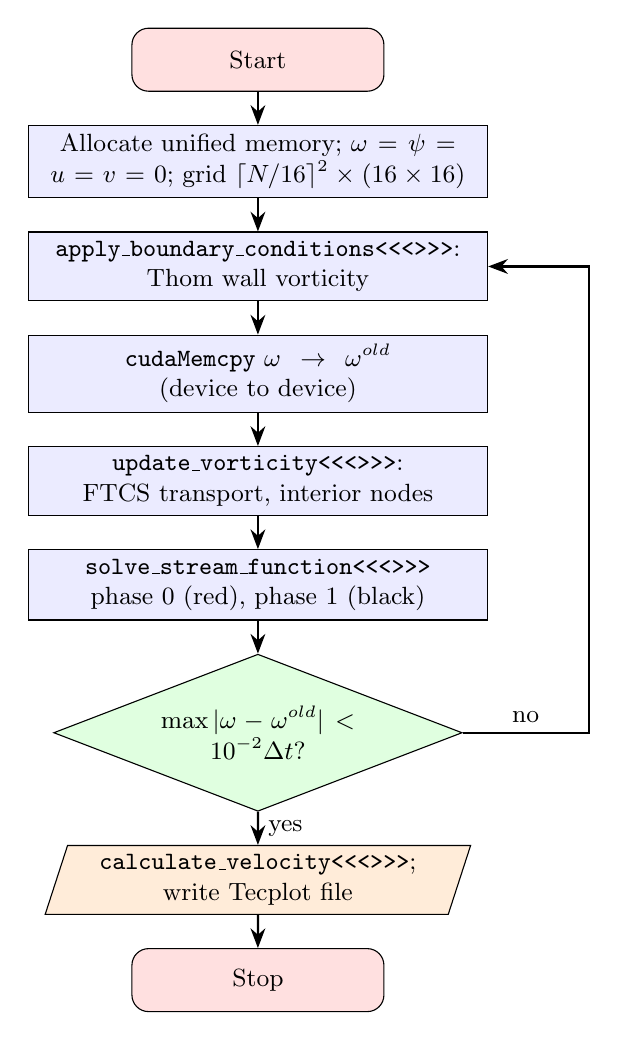
\begin{tikzpicture}[node distance=0.42cm]
\node(s)[startstop]{Start};
\node(i)[process,below=of s]{Allocate unified memory; $\omega=\psi=u=v=0$; grid $\lceil N/16\rceil^2\times(16\times16)$};
\node(bc)[process,below=of i]{\texttt{apply\_boundary\_conditions<<<>>>}: Thom wall vorticity};
\node(cp)[process,below=of bc]{\texttt{cudaMemcpy} $\omega\to\omega^{old}$ (device to device)};
\node(vt)[process,below=of cp]{\texttt{update\_vorticity<<<>>>}: FTCS transport, interior nodes};
\node(ps)[process,below=of vt]{\texttt{solve\_stream\_function<<<>>>} phase 0 (red), phase 1 (black)};
\node(d)[decision,below=of ps]{$\max|\omega-\omega^{old}|<10^{-2}\Delta t$?};
\node(o)[io,below=of d]{\texttt{calculate\_velocity<<<>>>}; write Tecplot file};
\node(e)[startstop,below=of o]{Stop};
\draw[arrow](s)--(i);\draw[arrow](i)--(bc);\draw[arrow](bc)--(cp);\draw[arrow](cp)--(vt);\draw[arrow](vt)--(ps);\draw[arrow](ps)--(d);
\draw[arrow](d)--node[right,font=\small]{yes}(o);\draw[arrow](o)--(e);
\draw[arrow](d.east)--node[above,font=\small]{no}++(1.6,0)|-(bc.east);
\end{tikzpicture}\caption{Time loop of \texttt{code/Lid\_driven\_Cavity.cu}; every box marked \texttt{<<<>>>} is a CUDA kernel with one thread per grid node.}\end{figure}

\subsection{Verification without a GPU: CPU emulation of the kernels}
The workspace used for this revision has no NVIDIA GPU, so the kernels were executed by a CUDA emulation layer (\texttt{tools/cuda\_cpu\_shim.h}, \texttt{tools/emulate.sh}). The script rewrites each launch \texttt{k<<<G,B>>>(args)} into a loop over \texttt{blockIdx} and \texttt{threadIdx} that calls the \emph{unmodified} kernel body once per thread, and maps \texttt{cudaMallocManaged}, \texttt{cudaMemcpy} and \texttt{cudaDeviceSynchronize} to their host equivalents. Because every kernel here writes disjoint data and reads only data not written in the same launch (the red--black split guarantees this for the stream-function sweep), sequential execution gives the same result as the GPU apart from floating-point contraction. The CPU times quoted below are therefore single-core baselines; \texttt{run.sh} builds the same source with \texttt{nvcc -O3 -arch=native} and runs it on the GPU when one is available (results in \texttt{results/run\_<N>\_gpu} and \texttt{results/timing.txt}).

\section{Code review of the submitted program}\label{sec:review}
The submitted file is kept as \texttt{original/Lid\_driven\_Cavity\_original.cu}; all changes are marked \texttt{[FIX]}, \texttt{[ADDED]} or \texttt{[CHANGED]} in \texttt{code/Lid\_driven\_Cavity.cu}. The numerical scheme and kernel structure were not altered.
\begin{table}[H]\centering\small
\begin{tabular}{p{3.6cm}p{11.6cm}}\toprule
Item & Error and correction\\\midrule
\texttt{\#define Dt 0.001} & With $h=0.0025$ the diffusion number is $d=1.6$, 6.4 times the limit $\Delta t\le h^2\mathrm{Re}/4=1.5625\times10^{-4}$ derived in the original notes; the emulated run overflows to \texttt{inf} within about 12 steps. Set to $1.5\times10^{-4}$ ($d=0.24$).\\
\texttt{\#define Error 1e-5} & The test is on $\max|\omega^{n+1}-\omega^n|=\Delta t\,|\partial\omega/\partial t|$; with the stable $\Delta t$ it stopped the $401^2$ run at $t=8.7$ while $\psi$ still lagged ($\max|\nabla^2\psi+\omega|=0.11$, $\psi_{min}$ 1.8\% off). Replaced by $10^{-2}\Delta t$, i.e.\ $|\partial\omega/\partial t|<10^{-2}$, identical to the original value at $\Delta t=10^{-3}$.\\
\texttt{MaxIter 50000} & $t_{max}=7.5$ at the stable time step, shorter than the transient; raised to 400\,000 (the convergence test ends the run).\\
\texttt{OUTPUT\_INTERVAL 1} & One 11 MB Tecplot file per step, about 550 GB for 50\,000 steps; set to 20\,000.\\
\texttt{write\_tecplot2D} & Index \texttt{j*nx+i} while the solver stores \texttt{i*NY+j}: every field was written transposed. Fixed.\\
\texttt{calculate\_velocity} & Index \texttt{j*NX+i} (differentiates $\psi$ along the wrong direction) and an early \texttt{return} for all boundary nodes that made the lid-velocity assignment unreachable. Fixed: consistent indexing, wall and lid values set explicitly.\\
final output & Final file named after \texttt{MaxIter}; now \texttt{flow\_999999.dat}.\\
additions & Wall-clock timing (\texttt{clock\_gettime}), convergence history file, progress print every 1000 steps.\\\bottomrule
\end{tabular}\caption{Errors found in the submitted code and their corrections.}\end{table}

\section{Results}
\subsection{Convergence history}
\begin{figure}[H]\centering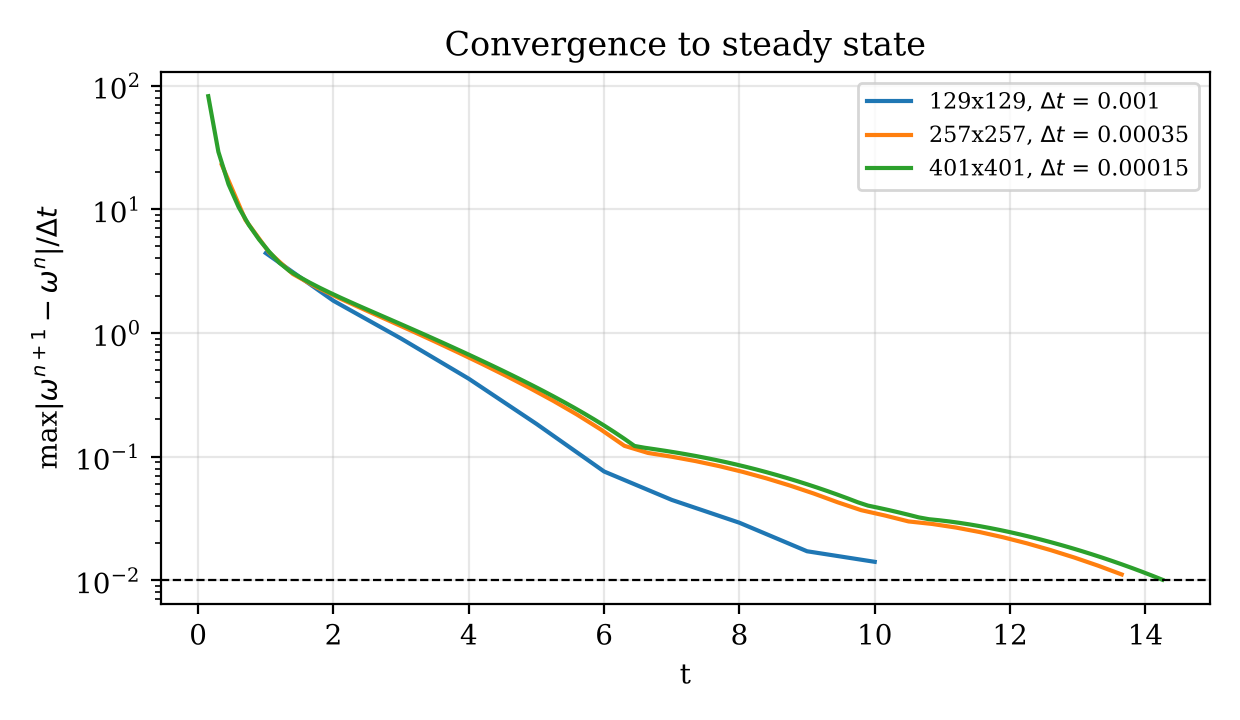
\includegraphics[width=0.72\textwidth]{../results/fig_convergence_history.png}
\caption{Rate of change of the vorticity, $\max|\omega^{n+1}-\omega^n|/\Delta t$, for the three grids (default stopping tolerance, dashed).}\end{figure}
After the start-up transient the residual decays exponentially. The finer grids decay more slowly because the stream-function lag $\tau_\psi$ grows with $\Delta t/h^2$, which is nearly constant here ($d\approx0.16$--$0.24$), so the number of steps grows roughly as $h^{-2}$.

\subsection{Flow field}
\begin{figure}[H]\centering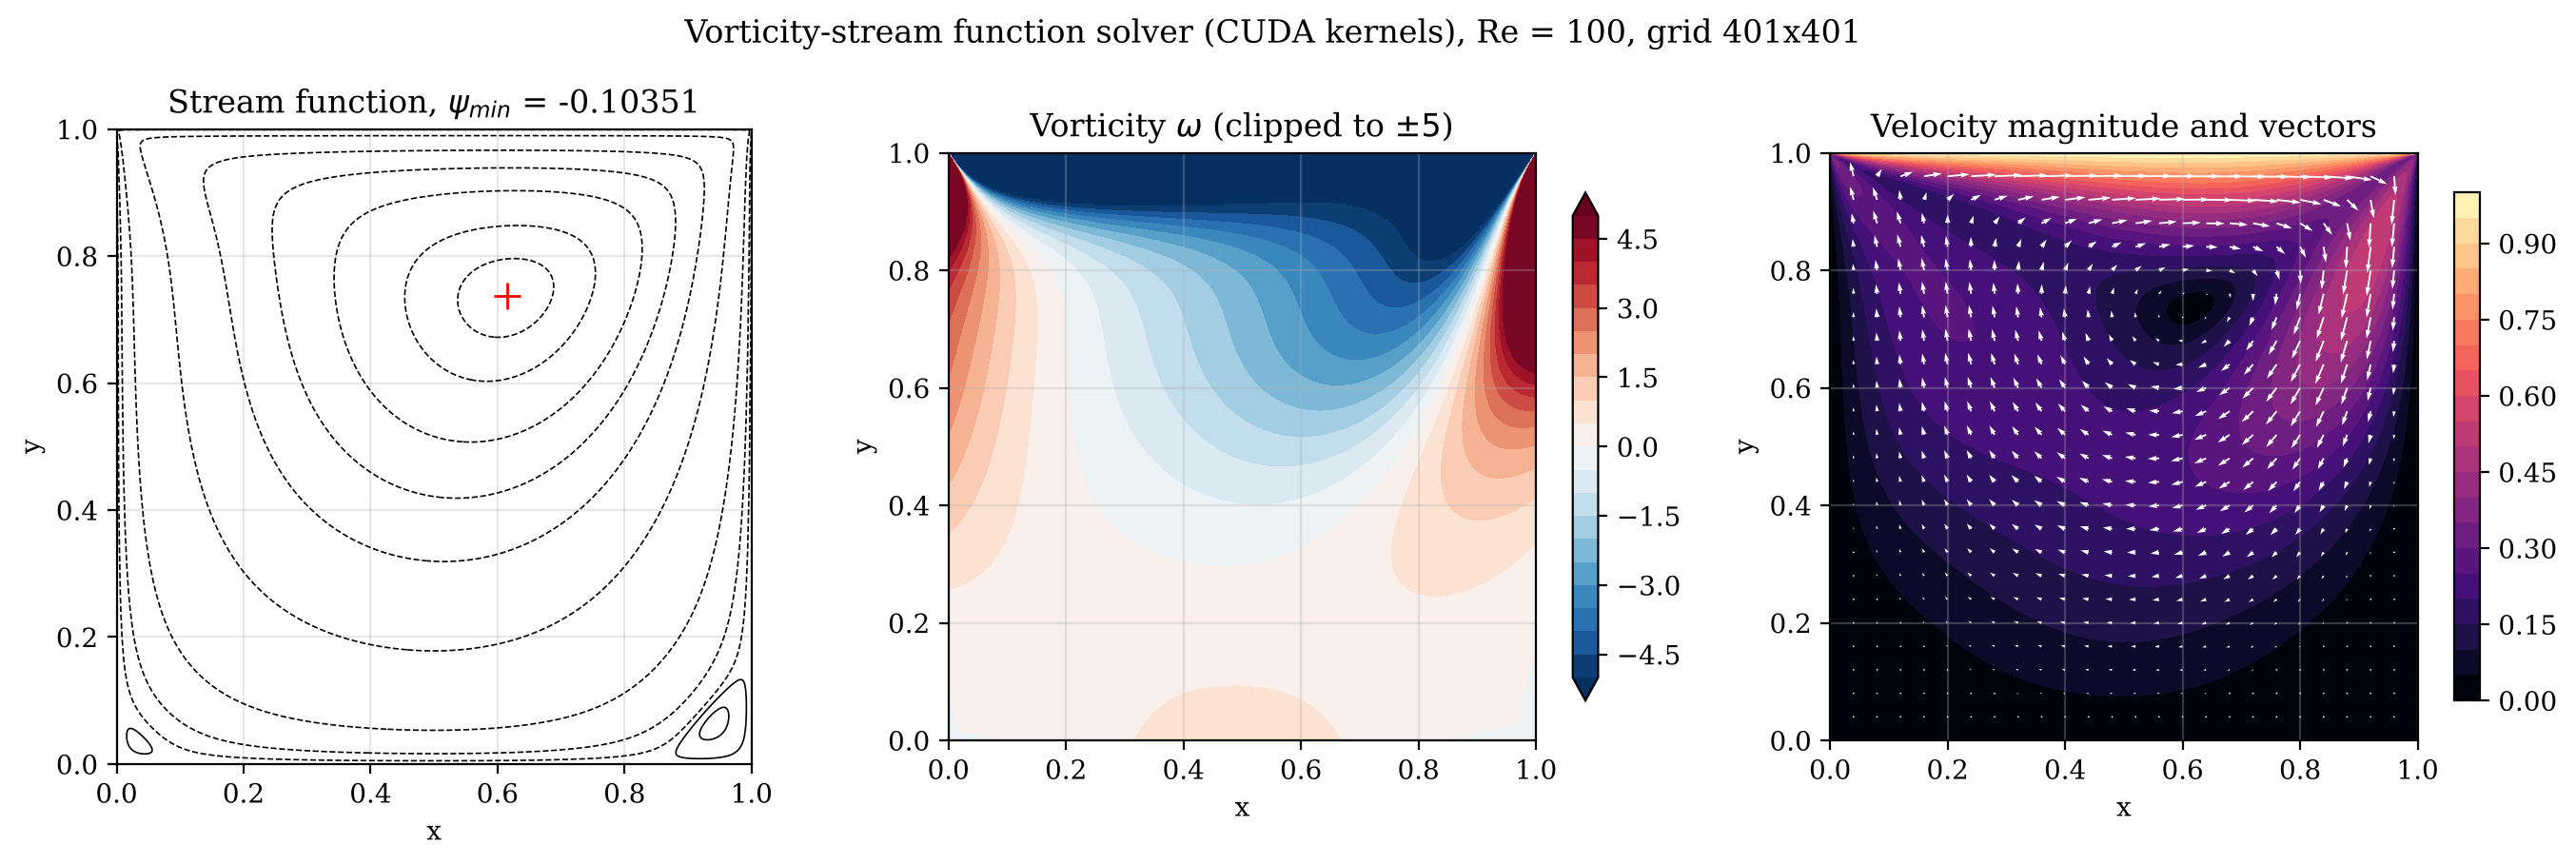
\includegraphics[width=\textwidth]{../results/fig_fields_401.png}
\caption{Stream function (vortex centre marked; contour levels down to $10^{-5}$ show both corner eddies), vorticity and velocity on the $401^2$ grid.}\end{figure}
The primary clockwise vortex sits above and downstream of the cavity centre. The vorticity is generated in the lid boundary layer and is singular at the two lid corners, where the velocity jumps from 1 to 0; vorticity of the opposite sign is produced on the downstream wall where the flow turns down. Two counter-rotating eddies occupy the bottom corners, four to five orders of magnitude weaker than the primary vortex.

\subsection{Comparison with Ghia, Ghia \& Shin (1982)}
\begin{figure}[H]\centering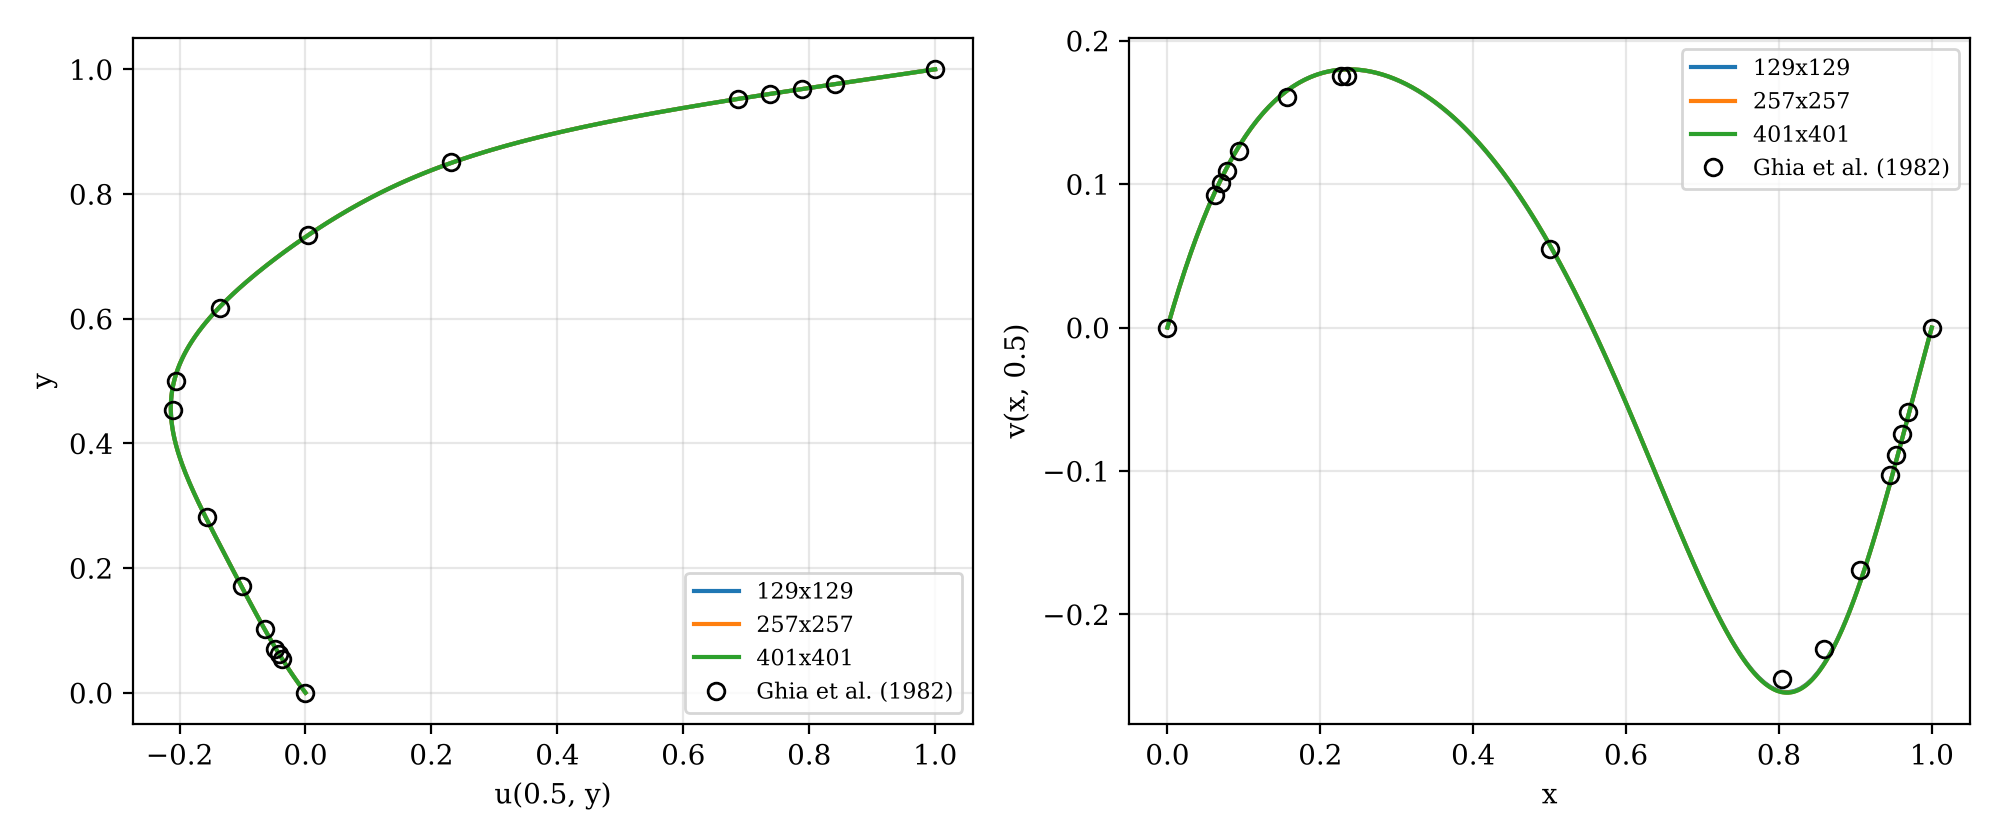
\includegraphics[width=\textwidth]{../results/fig_centreline_vs_ghia.png}
\caption{Centreline velocities $u(0.5,y)$ and $v(x,0.5)$ against the benchmark.}\end{figure}
\begin{table}[H]\centering\footnotesize\setlength{\tabcolsep}{4pt}
\resizebox{\textwidth}{!}{\begin{tabular}{lcccc}\toprule
Quantity & $129^2$ & $257^2$ & $401^2$ & Ghia et al.\\\midrule
$\psi_{min}$ & $-0.103335$ & $-0.103476$ & $-0.103503$ & $-0.103423$\\
centre $(x,y)$ (default runs) & (0.616, 0.737) & (0.616, 0.737) & (0.616, 0.737) & (0.617, 0.734)\\
$u_{min}$ on $x=0.5$ & $-0.213444$ & $-0.213896$ & $-0.213985$ & $-0.21090$\\
$v_{max}$ on $y=0.5$ & $0.178882$ & $0.179403$ & $0.179504$ & $0.17527$\\
$v_{min}$ on $y=0.5$ & $-0.252853$ & $-0.253565$ & $-0.253704$ & $-0.24533$\\
$\psi$ bottom-right / left eddy & $1.37\!\times\!10^{-5}$ / $2.07\!\times\!10^{-6}$ & $1.35\!\times\!10^{-5}$ / $1.94\!\times\!10^{-6}$ & $1.34\!\times\!10^{-5}$ / $1.90\!\times\!10^{-6}$ & $1.25\!\times\!10^{-5}$ / $1.75\!\times\!10^{-6}$\\
$\max|u-u_{Ghia}|$, $\max|v-v_{Ghia}|$ & 0.0049, 0.0097 & 0.0048, 0.0099 & 0.0048, 0.0100 & --\\\bottomrule
\end{tabular}}\caption{Benchmark quantities (extrema located to sub-grid accuracy by quadratic fits; extremum values from the tightly converged runs).}\end{table}
$\psi_{min}$ and the vortex centre agree with the benchmark to $0.08\%$ and within one grid cell of the benchmark grid. The centreline extrema differ from Ghia's tabulated values by $1.5$--$3.4\%$, and these differences do \emph{not} shrink with refinement: Ghia's values are samples on a $129\times129$ grid at fixed points (e.g.\ $v$ is tabulated at $x=0.8047$, whereas the minimum lies at $x=0.8105$), so the benchmark itself carries an error of this size. The grid study below shows that the present results are converged to much better than this.

\subsection{Grid convergence study}
Three grids with refinement ratios $r_{21}=1.5625$ and $r_{32}=2$ were run to the tight tolerance ($|\partial\omega/\partial t|<10^{-4}$, so that the residual transient does not contaminate the differences). The observed order $p$, the Richardson-extrapolated value and the fine-grid convergence index (GCI, safety factor 1.25) follow Celik et al.\ (2008):
\begin{equation}
p=\frac{1}{\ln r_{21}}\Big|\ln\Big|\frac{\varepsilon_{32}}{\varepsilon_{21}}\Big|+\ln\frac{r_{21}^p-s}{r_{32}^p-s}\Big|,\quad
\phi_{ext}=\frac{r_{21}^p\phi_1-\phi_2}{r_{21}^p-1},\quad
\mathrm{GCI}=\frac{1.25\,|(\phi_1-\phi_2)/\phi_1|}{r_{21}^p-1}.
\end{equation}
\begin{table}[H]\centering\small
\begin{tabular}{lccc}\toprule
Quantity & observed order $p$ & extrapolated value & GCI$_{fine}$ [\%]\\\midrule
$\psi_{min}$ & 2.02 & $-0.103522$ & 0.022\\
$u_{min}$ & 2.01 & $-0.214046$ & 0.036\\
$v_{max}$ & 2.02 & $0.179573$ & 0.048\\
$v_{min}$ & 2.01 & $-0.253801$ & 0.047\\\bottomrule
\end{tabular}\caption{Grid convergence (\texttt{results/grid\_study.txt}).}\end{table}
\begin{figure}[H]\centering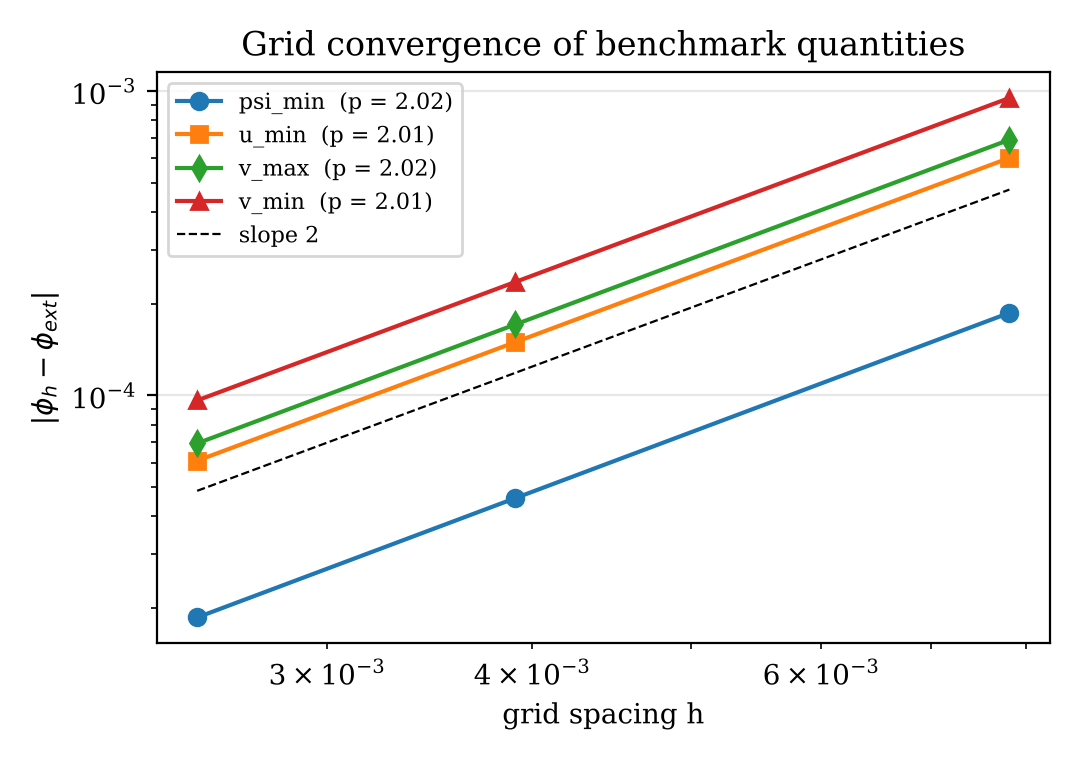
\includegraphics[width=0.6\textwidth]{../results/fig_grid_convergence.png}
\caption{Distance from the extrapolated value against grid spacing: all quantities converge at second order.}\end{figure}
The observed order matches the formal second order of the scheme, which also confirms that the Thom wall condition does not degrade the interior accuracy. The default stopping tolerance leaves a small transient error: on the $401^2$ grid $v_{max}$ is $0.18006$ with the default test and $0.17950$ with the tight one ($0.3\%$); for benchmark-quality numbers the tight tolerance (\texttt{bash run.sh study}) should be used.

\subsection{Run times}
\begin{table}[H]\centering\small
\begin{tabular}{lccc}\toprule
Grid & steps (default) & CPU emulation, 1 core [s] & per node and step [ns]\\\midrule
$129^2$ & 10\,940 & 3.4 & 19\\
$257^2$ & 39\,616 & 37.5 & 14\\
$401^2$ & 95\,127 & 710.6 & 46\\\bottomrule
\end{tabular}\caption{Serial CPU baseline (emulated kernels, \texttt{g++ -O3}). The GPU wall times are written by \texttt{run.sh} to \texttt{results/timing.txt} when the code is run on a machine with \texttt{nvcc} and an NVIDIA GPU.}\end{table}
The step count grows like $h^{-2}$ at constant $d$ and the work per step like $h^{-2}$, so the total cost grows like $h^{-4}$; this is the regime where the per-node parallelism of the GPU pays off, provided the per-step host reduction mentioned above is moved to the device.

\section{Conclusions}
\begin{itemize}
\item The CUDA vorticity--stream function solver, after correcting an unstable time step (6.4 times the diffusion limit that the original notes themselves derive), transposed array indexing in the output and velocity routines, a per-step output that would have written $\sim$550 GB, and a stopping test that ignored the time step, reproduces the $\mathrm{Re}=100$ cavity flow.
\item $\psi_{min}=-0.10350$ at $(0.616,0.737)$ agrees with Ghia et al.\ to $0.08\%$; both corner eddies are captured.
\item A three-grid study shows second-order convergence ($p=2.01$--$2.02$) with GCI $<0.05\%$; the extrapolated benchmark values are $\psi_{min}=-0.10352$, $u_{min}=-0.21405$, $v_{max}=0.17957$, $v_{min}=-0.25380$.
\item All kernels were verified by serial emulation; GPU timings are produced by \texttt{run.sh} on a CUDA-capable machine.
\end{itemize}

\section*{References}
\small
U.\ Ghia, K.N.\ Ghia, C.T.\ Shin, High-Re solutions for incompressible flow using the Navier--Stokes equations and a multigrid method, \emph{J.\ Comput.\ Phys.} 48 (1982) 387--411.\\
I.B.\ Celik, U.\ Ghia, P.J.\ Roache, C.J.\ Freitas, H.\ Coleman, P.E.\ Raad, Procedure for estimation and reporting of uncertainty due to discretization in CFD applications, \emph{J.\ Fluids Eng.} 130 (2008) 078001.\\
A.\ Thom, The flow past circular cylinders at low speeds, \emph{Proc.\ R.\ Soc.\ Lond.\ A} 141 (1933) 651--669.\\
H.\ Juuj\"arvi, I.\ Kinnunen, Lid driven cavity flow using stencil-based numerical methods (reference used in the original notes).\\
NVIDIA, \emph{CUDA C++ Programming Guide} (unified memory, thread hierarchy).
\normalsize
\section*{Reproducing the results}
\texttt{bash run.sh} (GPU if available, then CPU emulation of the $129^2$, $257^2$, $401^2$ grids, about 13 min on one core); \texttt{bash run.sh study} adds the tightly converged grid study (about 10 more minutes); \texttt{bash run.sh gpu} runs only the GPU cases. Post-processing: \texttt{python3 code/postprocess.py}.

\appendix\section{Source code}
\lstinputlisting[language=C++]{../code/Lid_driven_Cavity.cu}
\end{document}
